\chapter{Dataset and Marker Set}
A critical phase in our research is the creation of a relevant and high-quality dataset, 
as the quality of the dataset can significantly impact the outcomes of our research efforts.
Here, we detail the methodology used to collect the dataset and its constituents.
Our primary objective is to develop an automated method for detecting the initiation of full-body human movements and identifying the most effective predictive movement features.
Central to this research is capturing motion dynamics accurately.
The participation of these skilled dancers is crucial because their deep knowledge of body mechanics leads to precise and high-quality motion data.
This collaboration yields expressive movements with distinct starting points, aligning with research goals.
Their expertise increases dataset quality, providing a resource that encapsulates human motion intricacies accurately and artistically.

\section{Raw Data Sources}
\label{sec:dataset}
The dataset contains two categories of expressive movements, each associated with a different recording session.
The details of both types of movements are provided below.\\
These segments represents various participants performing simple movement sequences, which are captured from different angles using some cameras.
The videos are synchronized through SMPTE timecode and each video is accompanied by corresponding motion capture data that records the positions of body parts.
The systems used for the recording are different versions of the same software, the \textit{Qualisys Motion Capture system}.


\subsection{WhoLoDance Dataset}
This specific portion of the dataset was collected within the framework of the H2020-ICT-2015 EU Project named $WhoLoDance$.
during the month of March in 2016.
These recording sessions are primarily characterized by their multimodal nature, 
meaning that they involve the use of multiple data recording methods. 
The primary focus during these sessions was on capturing expressive aspects of movement, 
specifically qualities related to movement dynamics. These qualities encompassed various factors, 
including the origin of movement, lightness, fluidity, and more.
The participants in these sessions are professional dancers 
who prepared for their recording sessions by designing a series of exercises in advance. 
The recorded movements primarily revolved around contemporary dance techniques. 
Importantly, these movements were performed without any accompanying music to ensure that 
the dancers' performances were not influenced by external auditory cues.

\subsection{Montpellier - UniGe Dataset}
This specific subset of the dataset was captured during a collaborative project involving the University of Genova and the University of Montpellier in July 2020. 
These recording sessions are divided into two segments: individual actions and dual actions. 
The primary aim of these action categories is to identify the source or initiator of motion in purposeful movements.\\
\underline{Action: Grasping}\\
From the trials that entail individual actions we took some that involves an individual grasping a object. 
In this scenario, participants are positioned in a way that they are facing an object situated at a distance equal to the length 
of their shoulder and at an angle of 20 degrees in the outward direction from the front of their dominant shoulder. 
Participants are instructed to reach for the object with their dominant hand in a natural and spontaneous manner and then place it in front of their non-dominant side.\\
\underline{Action: Throwing}\\
Participants are instructed to perform a two-handed throw, where in one scenario, 
the participant throws the ball and retrieves it themselves, while in the other scenario, two participants throw the ball to each other. 
This was done to introduce greater movement diversity.
It is worth noting that, for the purpose of motion analysis, the receiver and the thrower are considered separately.

\section{Original Marker Set}
\label{sec:orig_markers}
Due to a four-year gap between the recording of the two distinct subsets of the dataset, 
some differences in marker technology have emerged. 
In particular, the WhoLoDance recordings feature a full marker set consisting of 64 reflective markers. 
In contrast, the Montpellier-Unige recordings utilize the newer Qualisys sport marker set, comprising 41 markers. 
Nevertheless, the fundamental principles guiding the marker placement and grouping remain consistent for both datasets. 
The following figures (Figure \ref{fig:64markers}, Figure \ref{fig:41markers}) represent the body mapping of the different markers set. 

\begin{figure}[H]
    \centering
    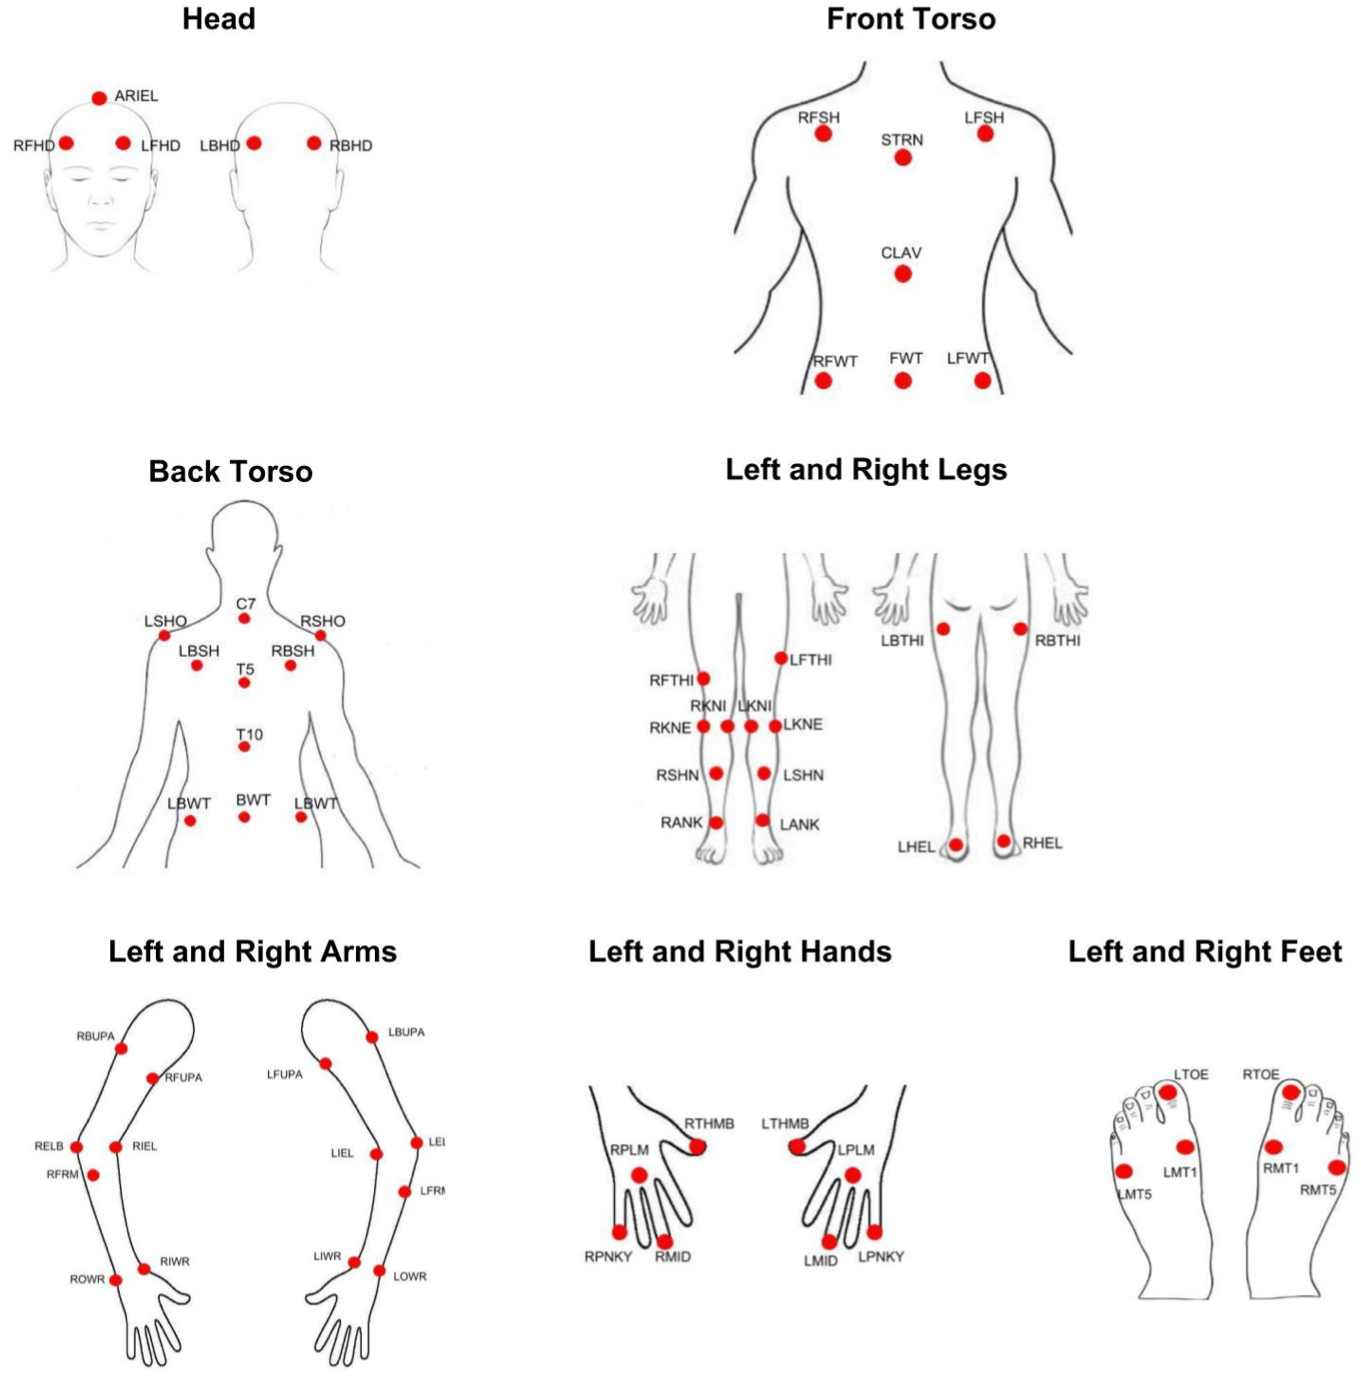
\includegraphics[width=\textwidth]{full_marker_set.png}
    \caption{Markers Set with 64 Labels}
    \label{fig:64markers}
\end{figure}

\begin{figure}[H]
    \centering
    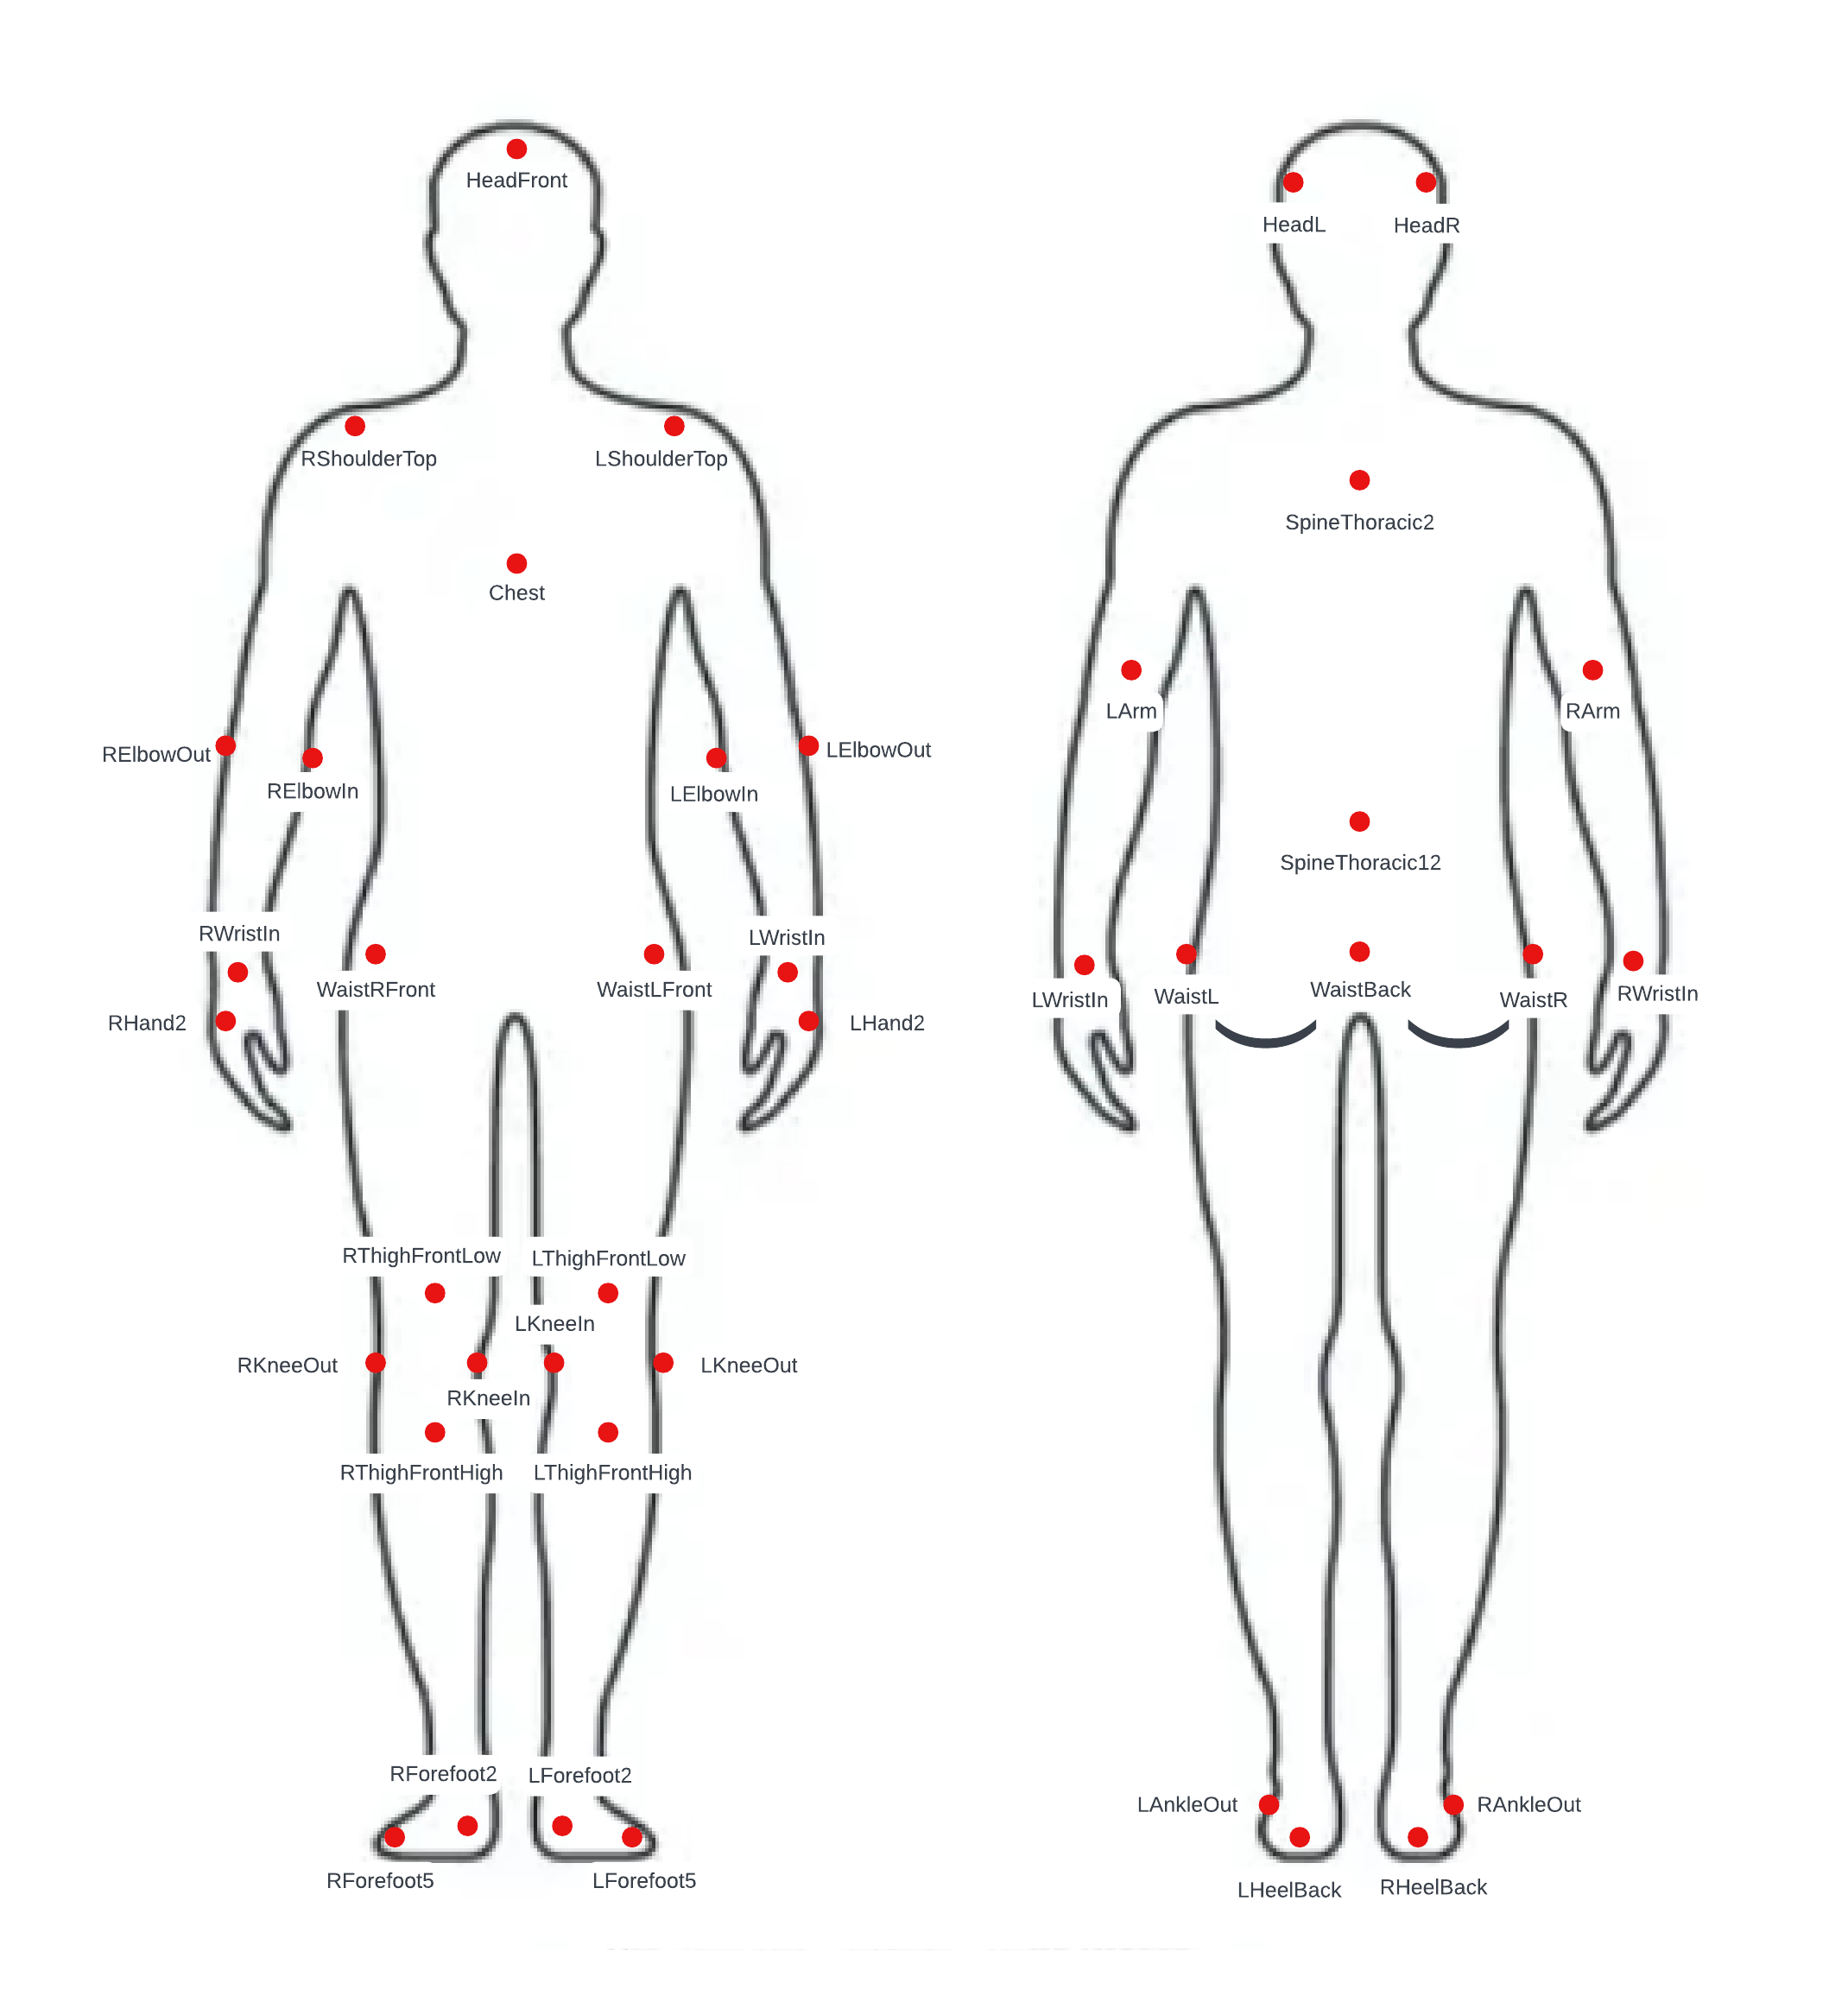
\includegraphics[width=\textwidth]{41Markers.png}
    \caption{Markers Set with 41 Labels}
    \label{fig:41markers}
\end{figure}

\section{Reduced Marker Set}
\label{sec:reduced_markers}
Firstly, we standardized the marker labels following the 64-marker scheme, 
we renamed some of the 41-marker labels to align with the full version (Table \ref{tab:marker_mapping_41}).

The reduced marker set is achieved by reducing the count of markers employed from the full marker set.
This because a simplified skeletal framework can adeptly communicate essential insights about expressive movements.
The reduction of multiple markers into individual joints is implemented to mitigate the possibility of marker omission. \\
This reduction was performed by computing the $barycentre$ of grouped joints (following the grouping scheme provided in Table \ref{tab:marker_mapping_64}) as follows:
\begin{enumerate}
    \item Extract the $x$, $y$, $z$ $coordinates$ for each marker of the cluster.
    \item Compute for each of $x$, $y$, $z$ their average, by summing all the $x$-markers together
    (and similarly for $y$ and $z$) and then dividing by the number of markers in the cluster.
\end{enumerate} 

\begin{table}[H]
    \centering
    \begin{tabular}{||c||c||}
    \hline
    \textbf{41 Sport Marker Set Labels} & \textbf{64 Marker Set Labels} \\
    \hline
    RKneeIn, LKneeIn & RKNI, LKNI \\
    HeadFront, HeadL, HeadR & ARIEL, LFHD, RFHD \\
    Chest & STRN \\
    WaistLFront, WaistRFront & LFWT, RFWT \\
    LShoulderTop, RShoulderTop & LSHO, RSHO \\
    SpineThoracic2, SpineThoracic12 & C7, T10 \\
    WaistBack, WaistL, WaistR & BWT, LBWT, RBWT \\
    LKneeOut, RKneeOut & LKNE, RKNE \\
    LHeelBack, RHeelBack & LHEL, RHEL \\
    LAnkleOut, RAnkleOut & LANK, RANK \\
    LForefoot2, LForefoot5, RForefoot2, RForefoot5& LTOE, LMT5, RTOE, RMT5\\
    LHand2, RHand2 & LPLM, RPLM \\
    LWristIn, LWristOut, RWristIn, RWristOut & LIWR, LOWR, RIWR, ROWR \\
    LElbowIn, LElbowOut, RElbowIn, RElbowOut & LIEL, LELB, RIEL, RELB \\
    \hline
    \end{tabular}
    \caption{41 Markers renaming convention}
    \label{tab:marker_mapping_41}
\end{table}

\begin{table}[H]
    \centering
    \begin{tabular}{||c||c||}
        \hline
        \textbf{Reduced Marker Set Labels} & \textbf{Partition of the 64 Marker Set Labels} \\
        \hline
        right\_foot & RHEL, RMT1, RMT5, RTOE \\
        left\_foot & LHEL, LMT1, LMT5, LTOE \\
        right\_ankle & RANK \\
        left\_ankle & LANK \\
        right\_knee & RKNE, RKNI \\
        left\_knee & LKNE, LKNI \\
        right\_hip & RFWT, RBWT \\
        hip\_center & RFWT, LFWT, RBWT, LBWT \\
        left\_hip & LFWT, LBWT \\
        spine & C6, C7, T5, T10, BWT, STRN, CLAV, FWT \\
        right\_hand & RPLM, RTHMB, RINDX, RMID, RPNKY\\
        left\_hand & LPLM, LTHMB, LINDX, LMID, LPNKY \\
        right\_wrist & ROWR, RIWR \\
        left\_wrist & LOWR, LIWR \\
        right\_elbow & RELB, RIEL, RFRM\\
        left\_elbow & LELB, LIEL, LFRM \\
        right\_shoulder & RSHO \\
        shoulder\_center & LSHO, RSHO \\
        left\_shoulder & LSHO \\
        head & RBHD, LBHD, LFHD, RFHD, ARIEL \\
        \hline
    \end{tabular}
    \caption{Mapping of the full marker set to the reduced marker set}
    \label{tab:marker_mapping_64}
\end{table}

\section{Annotations}
\label{sec:annotations}
Starting from the recordings of movements from these sources, we selected about one hundred segments in which we could clearly identify the origin of the movement.\\
Each video fragment was given a label corresponding to the edge between two joints that was deemed to be the origin of the movement.\\
The labelling process was carried out by individually labelling half of the segments. Then we compared our labels and considered for our dataset only those on which we agreed without any a-priori knowledge on the other's opinion.
We proposed those labels to our professors and considered for the dataset only those on which all of us agreed.
The final selection was made merging our labels with the opinion of an expert dancer.\\
This process was used to include only the segments where the labelling was more certain and evident.\\ 

The ending result comprises an amount of 60 fragments, divided between 58 recordings coming from the "WhoLoDance" and 2 from the "Montpellier - Unige" session. 
It spaced over 15 of the 20 joints available, the others are discarted during refinement process.
Unfortunately, the dataset obtained ended up being unbalanced, meaning that there are some labels that are very frequent, some that are infrequent, and some labels that are completely absent.
In Figure \ref{fig:dataset_distribution} we can see the resulting distribution of each edge as the origin of movement.\\

\begin{figure}[H]
    \centering
    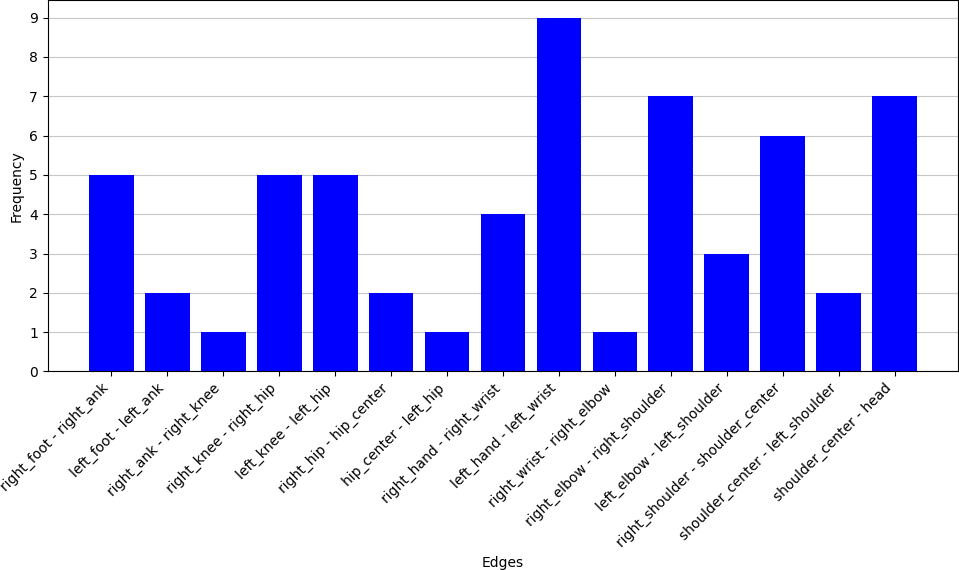
\includegraphics[width=\textwidth]{datasetDistribution.png}
    \caption{Edges frequencies in the Dataset}
    \label{fig:dataset_distribution}
\end{figure}